\providecommand\ExamFontPath{../../../字体/}
\documentclass[fontset=exam]{exam-zh}
\usepackage{longtable,booktabs,array,calc,multirow,fvextra}
\usepackage[normalem]{ulem}
\providecommand{\hl}[1]{#1}
\providecommand{\ul}[1]{\uline{#1}}
\DefineVerbatimEnvironment{verbatim}{Verbatim}{breaklines=true,fontsize=\small}
\providecommand{\tightlist}{\setlength{\itemsep}{0pt}\setlength{\parskip}{0pt}}
\newcommand{\pandocbounded}[1]{#1}
\setlength{\emergencystretch}{3em}
\setlength{\tabcolsep}{2pt}
\examsetup{page/size=a4paper}
\title{安徽大学 2004—2005 年 期末考试 A 卷}
\subject[4em]{离散数学}
\begin{document}
\maketitle
\fancyfoot[C]{第 \thepage 页（共 \pageref*{LastPage} 页）}
\noindent\makebox[\linewidth][c]{2004—2005 学年第二学期}\par
\pdfbookmark[1]{一、单项选择}{section72}

\par\medskip{\heiti

一、单项选择

\par}\smallskip

1 在自然数集\(N\)上，下列哪种运算是可结合的？（ ）

\begin{quote}
A. \(a*b = a - b\) B. \(a*b = max\{ a,b\}\)

C. \(a*b = a + 2b\) D. \(a*b = a \cdot b(mod3)\)
\end{quote}

2 下列代数系统\textless{}\(S\)，*\textgreater 中，哪个是群？（ ）

\begin{quote}
A. \(S = \{ 0,1,3,5\}\)，*是模 7 加法 B. \(S = Q\)（有理数集合），*是一般乘法
\end{quote}

C. \(S = Z\)（整数集合），*是一般减法 D. \(S = \{ 1,3,4,5,9\}\)，*是模 11 乘法

3 若\textless{}\(H\)，*\textgreater 是\textless{}\(G\)，*\textgreater 的真子群，且\(|H| = n\)，\(|G| = m\)，则有（ ）。

\begin{quote}
A. \(n\)整除\(m\) B. \(m\)整除\(n\)

C. \(n\)整除\(m\)且 \(m\)整除\(n\) D. \(n\)不整除\(m\)且 \(m\)不整除\(n\)
\end{quote}

4 下面哪个集合关于指定的运算构成环？（ ）

\begin{quote}
A. \(\{ a + b\sqrt[3]{2}|a,b \in Z\}\)，关于数的加法和乘法

B.\(\{ n\)阶实数矩阵\(\}\)，关于矩阵的加法和乘法
\end{quote}

C. \(\{ a + b\sqrt{2}|a,b \in Z\}\)，关于数的加法和乘法

D. \(\left\{ {\left. \begin{pmatrix}
a & b \\
b & a
\end{pmatrix} \right|a,b \in Z} \right\}\)，关于矩阵的加法和乘法

5 在代数系统中，整环和域的关系为（ ）。

\begin{quote}
A. 域一定是整环 B.域不一定是整环
\end{quote}

C. 整环一定是域 D. 域一定不是整环

6 \(N\)是自然数集，\(\leq\)是小于等于关系，则\((N, \leq )\)是（ ）。

\begin{quote}
A. 有界格 B.有补格 C. 分配格 D. 有补分配格
\end{quote}

7 图 1-1 给出的哈斯图表示的格中哪个元素无补元？（ ）

A. \(a\) B. \(c\) C. \(e\) D. \(f\) 图 1-1

\par\medskip{\centering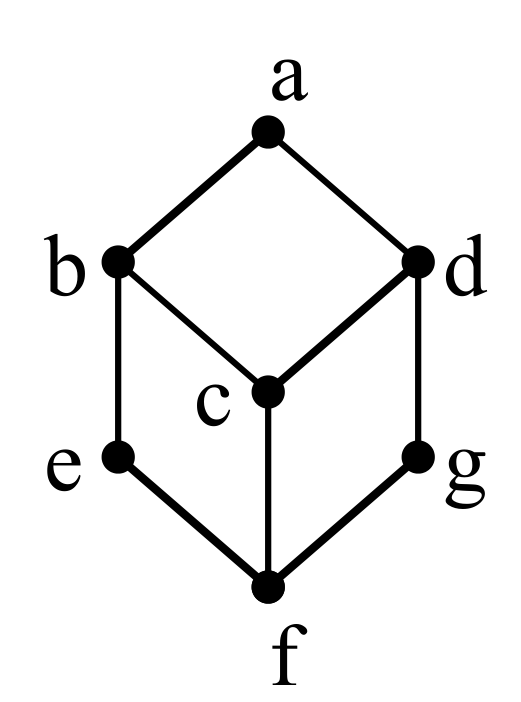
\includegraphics[width=5cm,height=4cm,keepaspectratio]{figures/hasse1.png}\par}\medskip

8 给定下列序列，可构成无向简单图的结点度数序列的是（ ）。

A.（1，1，2，2，3） B.（1，3，4，4，5）

C.（0，1，3，3，3） D.（1，1，2，2，2）

9 欧拉回路是（ ）。

A.路径 B.简单回路

C.既是基本回路也是简单回路 D.既非基本回路也非简单回路

10 哈密尔顿回路是（ ）。

A.路径 B.简单回路

C.既是基本回路也是简单回路 D.既非基本回路也非简单回路

\pdfbookmark[1]{二、填空题（以下每个下划线为一空，请按要求填入合适的内容。每空2分，共30分）。}{section100}

\par\medskip{\heiti

二、填空题（以下每个下划线为一空，请按要求填入合适的内容。每空 2 分，共 30 分）。

\par}\smallskip

1 设\(S\)是非空有限集，代数系统\((P(S), \cup , \cap )\)中，\(P(S)\)对\(\cup\)运算的单位元是\ul{＿＿＿＿}，零元是\ul{＿＿＿＿}，\(P(S)\)对\(\cap\)运算的单位元是\ul{＿＿＿＿}。

2 在运算表 2-1 中空白处填入适当符号，使\((\{ a,b,c\}, \circ )\)成为群。

①\ul{＿＿＿＿}，②\ul{＿＿＿＿}，③\ul{＿＿＿＿}，④\ul{＿＿＿＿}。

\begin{center}\begin{tabular}{c|ccc}$\circ$&$a$&$b$&$c$\\\hline$a$&\underline{①}&$a$&\underline{②}\\$b$&$a$&$b$&$c$\\$c$&\underline{③}&$c$&\underline{④}\end{tabular}\end{center}

3 设\(H = \{ 0,4,8\}\)，\(< H, +_{12} >\)是群\(< N_{12}, +_{12} >\)的子群，其中

\(N_{12} = \{ 0,1,2, \cdot \cdot \cdot ,11\}\)，\(+_{12}\)是模 12 加法，则\(< N_{12}, +_{12} >\)有\ul{＿＿＿＿}

个真子群，\(H\)的左陪集\(3H =\)\ul{＿＿＿＿}，\(4H =\)\ul{＿＿＿＿}。

4 设\(< A, \vee , \land , - >\)是一个布尔代数，如果在\(A\)上定义二元运算\(\oplus\)为：

\begin{quote}
\(a \oplus b = (a \land b) \vee (\overline{a} \land b)\)，则\(< A, \oplus >\)是一个\ul{＿ ＿ ＿＿}。 表 2-1
\end{quote}

5 任何一个具有\(2^{n}\)个元素的有限布尔代数都是\ul{＿ ＿＿＿}。

6 若连通平面图\(G\)有 4 个结点，3 个面，则\(G\)有\ul{＿＿ ＿＿}条边。

7 一棵树有两个结点度数为 2，一个结点度数为 3，三个结点度数为 4，它有\ul{＿ ＿＿＿}个度数为 1 的结点。

8 无向图\(G\)是由\(k\)（\(k \geq 2\)）棵数组成的森林，至少要添加\ul{＿＿ ＿＿}条边才能使\(G\)成为一棵树。

\pdfbookmark[1]{三、求解题（20分）}{section113}

\par\medskip{\heiti

三、求解题（20 分）

\par}\smallskip

1 试写出\(< N_{6}, +_{6} >\)中每个子群及其相应的左陪集。 （6 分）

2 若一个有向图\(G\)是欧拉图，它是否一定是强连通的？若一个有向图\(G\)是强连通的，它是否一定是欧拉图？说明理由。 （6 分）

3 有向图\(G\)如图 3-1 所示。

\par\medskip{\centering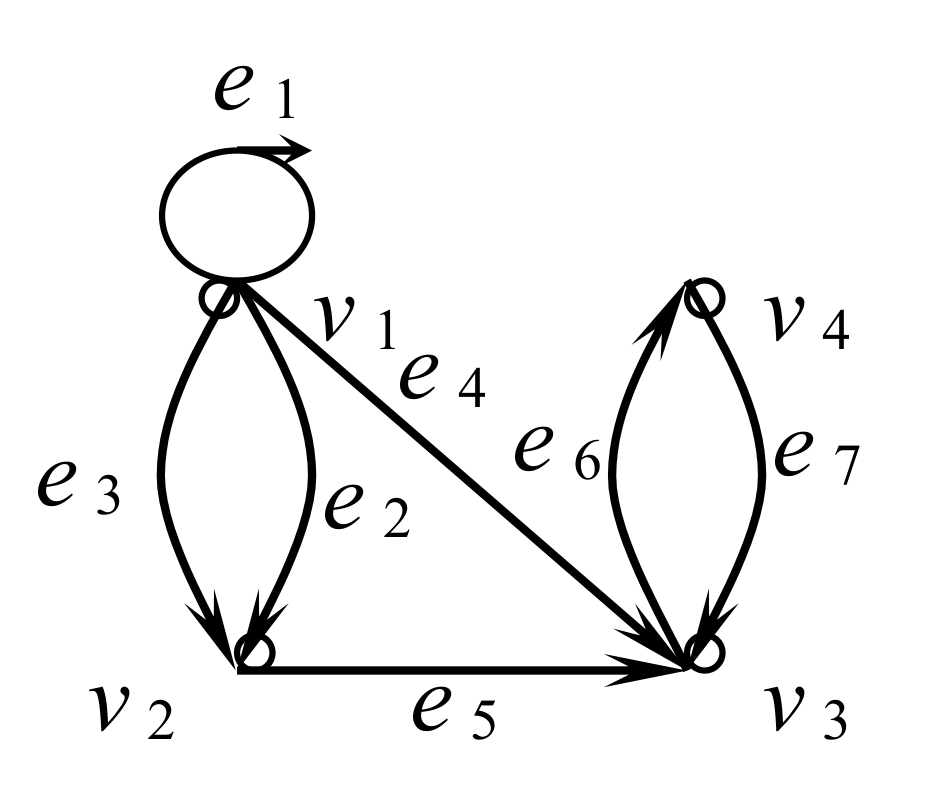
\includegraphics[width=5cm,height=4cm,keepaspectratio]{figures/digraph31.png}\par}\medskip

（1）求\(G\)的邻接矩阵\(A\)； （2 分）

（2）\(G\)中\(v_{1}\)到\(v_{4}\)长度为 4 的路径有几条？ （2 分）

（3）\(G\)中\(v_{1}\)到自身长度为 3 的回路有几条？ （2 分）

（4）\(G\)是哪类连通图？ （2 分）

图 3-1

\pdfbookmark[1]{四、证明题（30分）}{section122}

\par\medskip{\heiti

四、证明题（30 分）

\par}\smallskip

1 设\(< G,* >\)是一群，\(x \in G\)。定义：\(a \circ b = a*x*b\)，\(\forall a,b \in G\)。证明\(< G, \circ >\)也是一群。

2 证明：（1）证明在格中成立：\((a*b) \oplus (c*d) \leq (a \oplus c)*(b \oplus d)\)。 （5 分）

（2）证明布尔恒等式：\((a*c) \oplus (a'*b) \oplus (b*c) = (a*c) \oplus (a'*b)\)。 （5 分）

3 证明：（1）在 6 个结点 12 条边的连通平面简单图中，每个面由 3 条边围成。 （5 分）

（2）证明当每个结点的度数大于等于 3 时，不存在有 7 条边的简单连通平面图。

\end{document}
